\documentclass[11pt]{article}
\usepackage[utf8]{inputenc}\usepackage[T1]{fontenc}\usepackage{mathptmx}\usepackage[margin=1in]{geometry}
\usepackage{graphicx,booktabs,amsmath,amssymb,microtype,xcolor,caption}
\usepackage[hidelinks]{hyperref}
\DeclareUnicodeCharacter{2265}{\ensuremath{\geq}}\DeclareUnicodeCharacter{2264}{\ensuremath{\leq}}\DeclareUnicodeCharacter{00B1}{\ensuremath{\pm}}
\DeclareUnicodeCharacter{2192}{\ensuremath{\rightarrow}}\DeclareUnicodeCharacter{00D7}{\ensuremath{\times}}\DeclareUnicodeCharacter{2212}{\ensuremath{-}}
\providecommand{\tightlist}{\setlength{\itemsep}{0pt}\setlength{\parskip}{0pt}}
\emergencystretch=2em\captionsetup{font=small}
\title{The Babel Effect: Cross-Lingual Causal Profiles of Factual Recall in Two Small Language Models}
\author{Anonymous authors}
\date{Draft v2}
\begin{document}\maketitle
\begin{abstract}
Do language models store a fact once, in a language-neutral form, or separately per language? We trace the causal effect of restoring clean activations when the subject of a factual prompt is corrupted, in English (EN), Spanish (ES) and Hindi (HI), for Llama-3.2-3B-Instruct (92 facts) and Gemma-2-2B (58 facts), and compare per-layer profiles with a shuffled-fact permutation null. English and Spanish profiles of the same fact are aligned beyond chance in both models (MLP-profile cosine z = 4.22 and 4.81, p = 0.001). Hindi overlap is weaker: with a pooled null, Llama\textquotesingle s EN-HI and ES-HI pairs are above chance (z = 2.45, 2.47) and Gemma\textquotesingle s EN-HI marginally so (z = 2.19), but with a null restricted to the same relation only EN-ES remains significant after correction in both models. The weakness depends partly on Hindi subject length: with short Hindi subject spans the EN-HI cosine is 0.60 (Llama) against 0.20 with long spans. The layer where the fact is looked up is model-dependent (median layer 3 in Llama, 6 in Gemma). Edit transfer over every layer depends on the model: in Gemma mid-layer edits transfer more to Spanish and Hindi than early-layer edits, in Llama the opposite holds for Spanish, and Hindi transfer is small in both. The alignment is robust to rewording (within-language profile cosine exceeds the cross-language cosine in both models) and, in Llama, holds on 104 facts whose answers are not copyable across languages (EN-ES z = 4.87); an English statement in the prompt changes Spanish and Hindi answers in Llama more often than the weight edit does. Controls added after review show that the English-Spanish alignment survives centring of the profiles and entity clustering in both models, but in Llama it is concentrated in facts whose English and Spanish subject names are similar. The evidence is consistent with partly shared lookup for English and Spanish in Gemma, cannot be separated from subject-name overlap in Llama, and gives no support for a single language-agnostic space.
\end{abstract}
\section{Introduction}
Multilingual language models answer factual questions in many languages, yet it is unclear whether a fact is stored once and read out through language-specific front and back ends, or stored separately per language. The answer determines whether an edit made in one language should carry over to others. We test it with two measurements on open-weight models that fit one 8 GB GPU: overlap of causal-tracing profiles across languages, and transfer of a localised edit from English to Spanish and Hindi.

Contributions: (i) a cross-lingual causal-tracing comparison with a shuffled-fact permutation null, a relation-stratified variant of it and a Hindi tokenisation diagnostic; (ii) results on two models with different lookup layers; (iii) an edit-transfer measurement over every layer, with robustness checks (rewording, non-copyable relations, an in-context baseline); (iv) a pre-registered design with logged deviations, all code, write-once run directories and a verifiable claim manifest.

\section{Related work}
\textbf{Locating and editing facts.} Causal tracing and rank-one editing of MLP weights follow Meng et al. (2022, ROME, arXiv:2202.05262) and its multi-edit extension MEMIT (Meng et al., 2022, arXiv:2210.07229). Geva et al. (2023, arXiv:2304.14767) describe recall as subject enrichment, relation propagation and attribute extraction. Hase et al. (2023, arXiv:2301.04213) find that the layer where tracing peaks does not reliably predict the best layer to edit, which motivates sweeping edit layers rather than relying on the traced layer. Gupta et al. (2024, arXiv:2403.07175) and Yang et al. (2024, arXiv:2406.11263) trace model collapse after ROME edits to implementation details, which is relevant to how damage is measured.

\textbf{Multilingual recall mechanisms.} Wendler et al. (2024, arXiv:2402.10588) report that Llama-2 middle layers decode towards English before language-specific output. Fierro et al. (2024, arXiv:2410.14387) use patching on XGLM, EuroLLM and mT5 and find subject enrichment to be language-independent and object extraction language-dependent. Zhang et al. (2024, arXiv:2406.16416) locate language-agnostic factual neurons mostly in middle layers. Wang et al. (2025, arXiv:2504.04264) study cross-lingual factual inconsistency in LLaMA2-7B and BLOOM-560M. Lu et al. (2025, arXiv:2505.20546) analyse the multilingual factual-recall pipeline of Llama-3.2-3B, the model used here, in English, French, Spanish, Chinese, Japanese and Korean, without editing and without Hindi. Schut et al. (2025, arXiv:2502.15603) report English-like internal decisions in multilingual models. Multilingual factual probes are provided by X-FACTR (arXiv:2010.06189) and mLAMA (arXiv:2102.00894).

\textbf{Cross-lingual knowledge editing.} Wang et al. (2023, arXiv:2309.08952) and Khandelwal et al. (2024, arXiv:2407.10275) find that parameter-based editing transfers poorly across languages while in-context editing transfers much better; Nie et al. (2024, arXiv:2406.17764) report in-context editing across 53 languages and a penalty for non-Latin scripts. Qi et al. (2023, arXiv:2310.10378) edit BLOOM-3b with ROME in English and find that the edit propagates to languages whose factual knowledge is more consistent with English, including Spanish. Banerjee et al. (2024, arXiv:2406.11139) apply ROME and MEMIT in English, Spanish, Hindi and five other languages on 7B models and report low portability across languages. Beniwal et al. (2024, arXiv:2401.10521) study cross-lingual editing in BLOOM, mBERT and XLM-RoBERTa, including Hindi. Durrani et al. (2025, arXiv:2505.14393) survey the area.

\textbf{Position of this work.} The studies above either trace or edit, mostly on 7B-class models, and none of them compares per-layer causal profiles across English, Spanish and Hindi against a shuffled-fact null and then measures edit transfer, specificity and damage over every layer on the same model. We searched for such a combination and did not find one; this is an absence in a bounded search, not proof that none exists.

\section{Method}
\textbf{Models.} Llama-3.2-3B-Instruct (28 layers) and Gemma-2-2B (26 layers, base model), bf16, TransformerLens 3.9.0 without weight processing; one 8 GB GPU (peak 7.5 GiB). Weights are byte-identical (SHA-256) to the official repositories. Gemma is a base model and Llama an Instruct model; this confound is not separable here. A third family (BLOOM-1b7, pre-registered as A10, to test whether the weak Hindi overlap is a tokenisation effect) had not been run when this draft was written.

\textbf{Facts and phrasings.} Hand-written EN/ES/HI facts in five relations (capital\_of, capital\_country, landmark\_city, invention\_inventor, event\_year; 408 candidates, 447 for Gemma after adding 39 events), three phrasings per fact and language. For each relation and language the three best of six answer-first templates are chosen on a 30-fact tuning set (per model). A fact is kept if the canonical phrasing begins with the answer (strict, after spelling normalisation) in all three languages and one other phrasing contains it in its first line. Kept: 93 (Llama: capital\_of 27, capital\_country 38, landmark\_city 6, invention\_inventor 0, event\_year 22) and 58 (Gemma: 11, 11, 6, 0, 30).

\textbf{Causal tracing.} Gaussian noise (sigma = 3 × pooled subject-embedding std, per-fact seed) is added to the subject-token embeddings. A clean activation is restored at one (layer, prompt token) site of the residual stream or MLP output, and the effect is the change in the teacher-forced log-probability of the whole answer relative to the corrupted run (full-answer scoring; the first-token variant is stored). A pair is valid if the answer probability falls below half its clean value and the total effect is positive (92 of 93 and 58 of 58 facts).

\textbf{Overlap.} Per fact and language pair, cosine and Spearman correlation of the 28 (or 26) layer MLP-output profile at each language\textquotesingle s own last subject token; statistic = median over facts; null = fact i in one language paired with a permuted fact in the other (1000 permutations; pooled across relations, and, as a post-hoc sensitivity analysis that becomes primary for later data, within relation); z and one-sided p from the null; 95\% CIs by 2000 bootstrap resamples of facts. Six primary tests per model (3 pairs x 2 statistics), Bonferroni alpha 0.0083.

\textbf{Editing.} Rank-1 update of the MLP down-projection (ROME-style) at every layer for 10 facts per model, English prompt only, fitted on the full new answer; transfer ratio, specificity (20 controls) and damage (perplexity ratio on 100 WikiText-2 test sentences) as in A5. An in-context baseline (A9) is run for comparison, and a follow-up edit run (20 further facts) uses the traced layer, L//2 and a random layer.

\textbf{Extra relations and rewording.} Two relations whose answers differ across languages (landmark\_country, city\_country) add 34 facts for Llama and one for Gemma (A9). Phrasings 1 and 2 are traced for the first 30 valid facts of each model to test robustness to wording (H8).

\section{Results}


\subsection{Overlap against the null}
Table\textasciitilde{}\ref{tab:main} gives the pre-registered overlap results and Figures\textasciitilde{}\ref{fig:fig1} and\textasciitilde{}\ref{fig:fig2} show the profiles and the overlap. English-Spanish overlap is the one result that survives every check. Within relation and after correction, only EN-ES remains significant in both models. Spearman statistics agree in direction (Llama EN-ES z = 5.15; Gemma EN-ES z = 4.55). Per relation with its own null the samples are small (6-38 facts) and mostly not significant (Llama capital\_country EN-ES z = 2.75, capital\_of 2.08, event\_year 0.91). On the 33 facts both models keep, EN-ES is above the null in both (Llama z = 1.88, Gemma z = 4.09) and EN-HI is at the null in both (z = −0.21, 0.55).

\begin{table}[t]\centering\small\begin{tabular}{llcccc}\toprule
model & pair & MLP cosine [95\% CI] & null mean & $z$ pooled & $z$ within relation \\\midrule
Llama ($n=92$) & EN-ES & 0.627 [0.557, 0.702] & 0.519 & 4.22 & 3.29 \\
 & EN-HI & 0.509 [0.335, 0.594] & 0.429 & 2.45 & 1.79 \\
 & ES-HI & 0.423 [0.313, 0.529] & 0.328 & 2.47 & 1.98 \\\addlinespace
Gemma ($n=58$) & EN-ES & 0.464 [0.329, 0.542] & 0.292 & 4.81 & 3.85 \\
 & EN-HI & 0.226 [0.168, 0.283] & 0.136 & 2.19 & 1.68 \\
 & ES-HI & 0.137 [0.014, 0.267] & 0.134 & 0.08 & $-0.45$ \\\bottomrule
\end{tabular}\caption{Pre-registered overlap analysis: median MLP-profile cosine across facts, shuffled-fact null mean, and $z$ against the pooled and the within-relation null.}\label{tab:main}\end{table}
\begin{figure}[t]\centering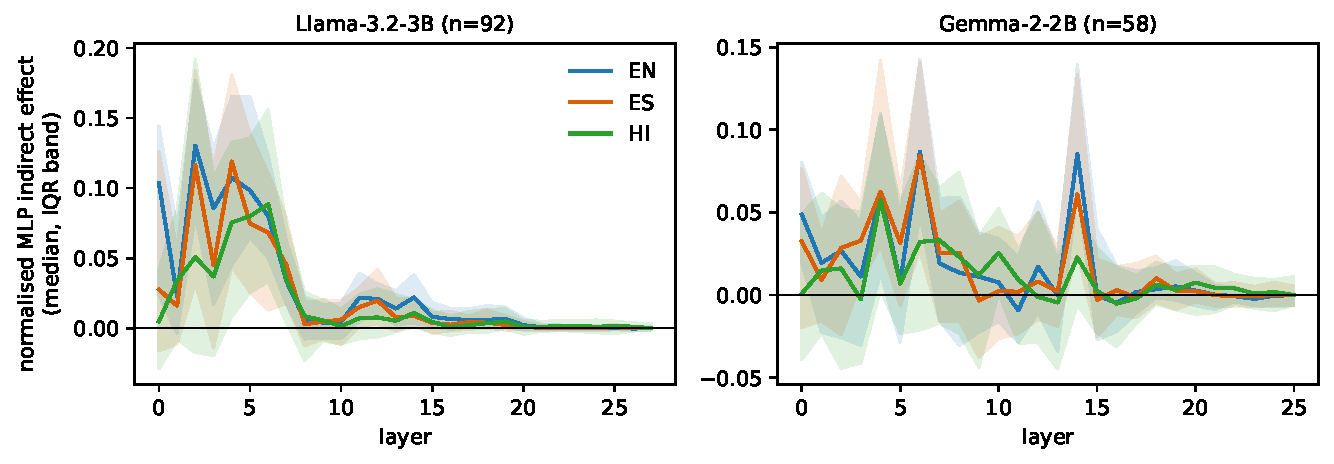
\includegraphics[width=0.95\linewidth]{figures/fig1_profiles.pdf}\caption{Median normalised MLP indirect effect per layer at each language's last subject token (band: interquartile range), for Llama-3.2-3B (left) and Gemma-2-2B (right).}\label{fig:fig1}\end{figure}
\begin{figure}[t]\centering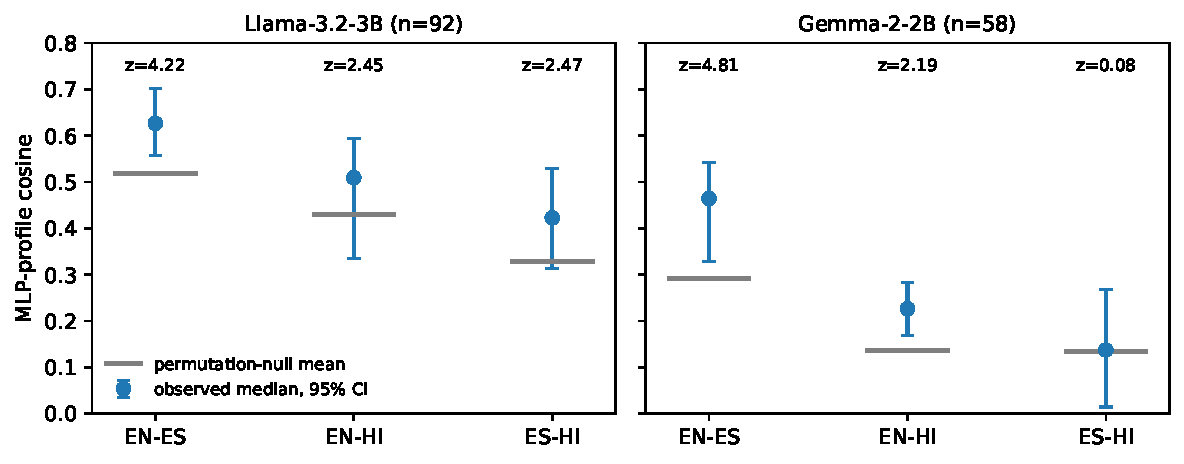
\includegraphics[width=0.95\linewidth]{figures/fig2_overlap.pdf}\caption{MLP-profile cosine between languages: observed median with 95\% bootstrap CI (dots) and mean of the shuffled-fact permutation null (bars).}\label{fig:fig2}\end{figure}
\begin{table}[t]\centering\small\begin{tabular}{llrccc}\toprule
model & set & $n$ & EN-ES & EN-HI & ES-HI \\\midrule
Llama-3.2-3B & all valid facts & 126 & 0.642 (5.06) & 0.500 (2.90) & 0.413 (2.63) \\
Llama-3.2-3B & non-copyable & 104 & 0.653 (4.87) & 0.529 (2.78) & 0.488 (3.51) \\
Llama-3.2-3B & all valid, stratified null & 126 & 0.642 (4.24) & 0.500 (2.66) & 0.413 (1.98) \\
\addlinespace
Gemma-2-2B & all valid facts & 59 & 0.436 (3.86) & 0.222 (2.09) & 0.132 (0.06) \\
Gemma-2-2B & non-copyable & 29 & 0.507 (2.53) & 0.314 (1.16) & 0.280 (0.42) \\
Gemma-2-2B & all valid, stratified null & 59 & 0.436 (3.18) & 0.222 (1.69) & 0.132 ($-$0.40) \\
\bottomrule\end{tabular}\caption{Extended overlap (with the added relations). Median MLP-profile cosine (z against the shuffled-fact null). Stratified: permutations within relation. Gemma gained one fact, so its non-copyable set ($n=29$) is below the pre-registered 50.}\label{tab:ext}\end{table}

\subsection{Where the fact is looked up}
The critical MLP layer (argmax at the last subject token) has median 3 (EN), 4 (ES), 4 (HI) in Llama (28 layers; 2-11\% of facts in layers 8-19) and 6, 6, 6 in Gemma (26 layers; 26-43\% in layers 8-19). The median absolute layer difference between languages is 2 in Llama and 2.5-4 in Gemma. The pre-registered expectation of a peak in layers 8-19 is not met for Llama. The median hides structure in Gemma (Figure\textasciitilde{}\ref{fig:fig4}, exploratory): the critical layer has modes at layers 4, 6 and 14; layer 14 holds the argmax for 17 of 58 English and 13 of 58 Spanish facts but for only 2 of 58 Hindi facts, and the cluster appears in three relations (English counts 3, 5, 9 in capital\_country, capital\_of, event\_year). Llama has no such late cluster (3\%, 2\%, 11\% of facts in layers 8-19 for EN, ES, HI).

\begin{figure}[t]\centering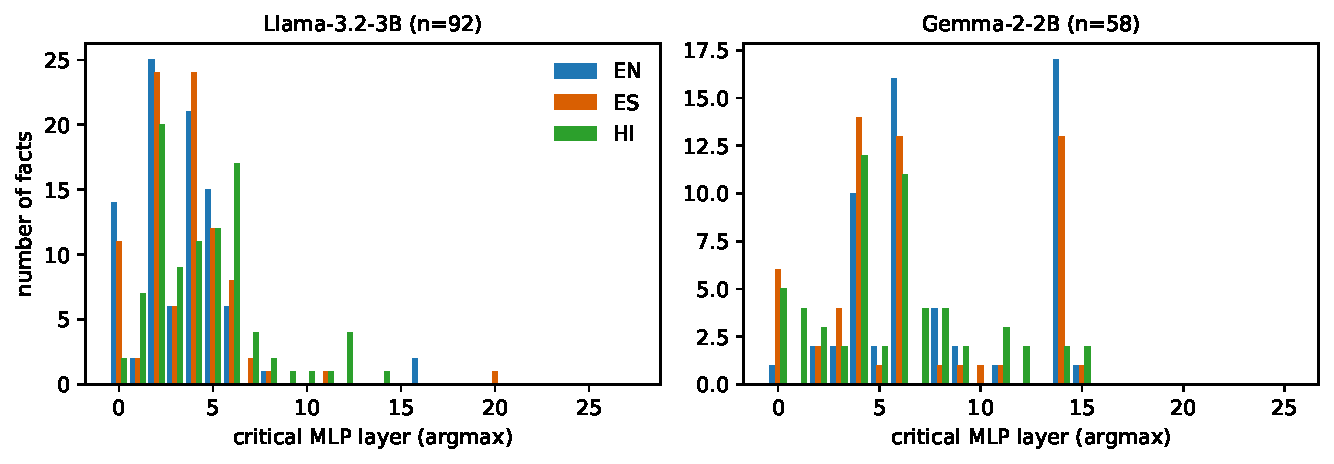
\includegraphics[width=0.95\linewidth]{figures/fig4_layer_hist.pdf}\caption{Distribution of the critical MLP layer (argmax of the profile) per language. Exploratory: Gemma shows modes at layers 4, 6 and 14.}\label{fig:fig4}\end{figure}

\subsection{Hindi tokenisation}
Hindi subjects span a median of 5 (Llama) and 8 (Gemma) tokens against 2 for English. The EN-HI profile cosine correlates negatively with Hindi subject span length (Spearman −0.35 Llama, −0.39 Gemma). Splitting at the median span, Llama\textquotesingle s EN-HI cosine is 0.597 for short spans (z = 1.69 pooled) and 0.199 for long spans (z = −1.22). So part of the weak Hindi result is a span-length effect; it does not explain it away, because EN-HI stays below EN-ES with short spans in both models. Hindi accuracy drops mainly for answers of 7 or more tokens (Figure\textasciitilde{}\ref{fig:fig3}; Llama 0.23 against 0.40-0.42; Gemma 0.02 against 0.21).

\begin{figure}[t]\centering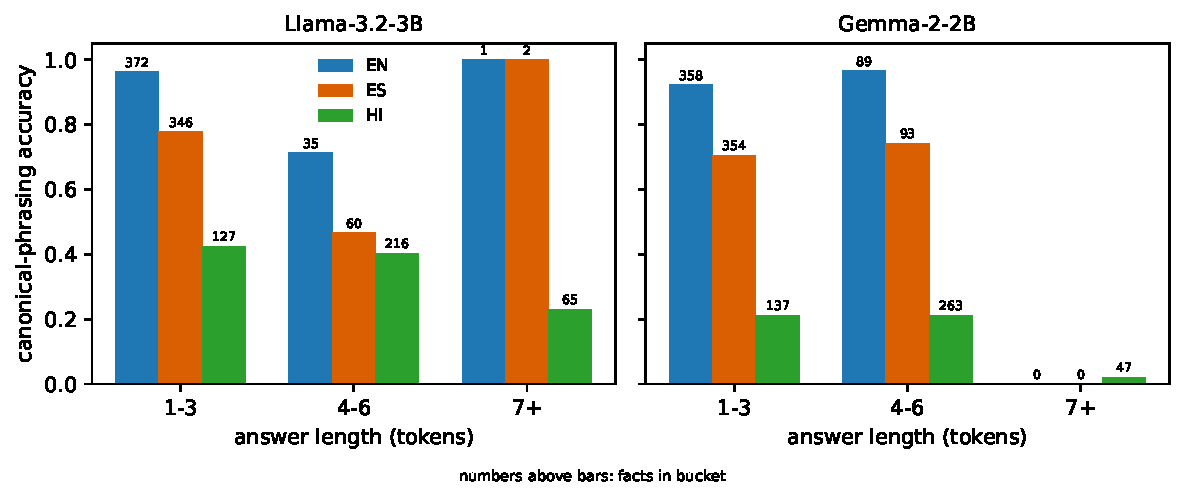
\includegraphics[width=0.95\linewidth]{figures/fig3_hindi.pdf}\caption{Canonical-phrasing accuracy by answer length in tokens, per language and model.}\label{fig:fig3}\end{figure}

\subsection{Edit transfer over layers}
For 10 facts per model (stratified by relation, English prompt only) we fitted a rank-1 edit of the MLP down-projection at every layer (280 edits in Llama, 260 in Gemma), toward a new object of the same relation, and scored greedy generation of the full new answer (Figures\textasciitilde{}\ref{fig:sw1} and\textasciitilde{}\ref{fig:sw2}). Per-layer rates rest on 10 facts and move in steps of 0.1.

\emph{English.} The edit makes the model produce the new answer for 84\% of Llama edits and 74\% of Gemma edits; it often fails at the last layers (final three layers: 53\% success in Llama, 20\% in Gemma). \emph{Transfer.} Averaged over all layers, the new answer appears in Spanish for 41\% (Llama) and 48\% (Gemma) of edits and in Hindi for 18\% and 20\%. Per layer, Hindi success never exceeds 0.5 (Llama layer 4; Gemma layers 12, 13, 17). \emph{Conditions (A5).} Table\textasciitilde{}\ref{tab:edit} lists the three conditions. At the fact\textquotesingle s English traced layer, English success is 0.9 in both models; median Spanish transfer ratio (dP\_ES / dP\_EN, over successful edits) is 0.66 in Llama and 0.38 in Gemma, and Hindi 0.0001 and 0.095. At L//2 (14 in Llama, 13 in Gemma) English success is 1.0 and 0.8, Spanish transfer 0.52 and 0.50, Hindi 0.010 and 0.016; specificity loss (maximum absolute probability change over 20 unrelated facts) is 0.084 and 0.089 against 0.030 and 0.027 at the traced layer. Median perplexity on 100 held-out sentences changes by at most 0.2\% (Llama) and 0.6\% (Gemma) at any layer. \emph{H7 (mid-layer edits transfer more than layers 0-5, and cost more specificity).} The result depends on the model. In Gemma, near-mid layers (L//2 ± 3) transfer more than layers 0-5 to Spanish (median paired difference +0.34, 95\% CI {[}0.01, 0.62{]}) and to Hindi (+0.07 {[}0.03, 0.13{]}) and lose more specificity (+0.04 {[}0.008, 0.19{]}); 8 of 10 and 9 of 10 facts have a positive Spanish and Hindi difference. In Llama the Spanish difference is negative (−0.31 {[}−0.47, −0.09{]}; 1 of 10 facts positive), the Hindi difference is negative or zero (−0.013 {[}−0.095, 0.000{]}) and the specificity difference includes zero (+0.004 {[}−0.023, 0.035{]}). H7 is therefore supported in Gemma and contradicted in Llama; we make no pooled claim.

\begin{figure}[t]\centering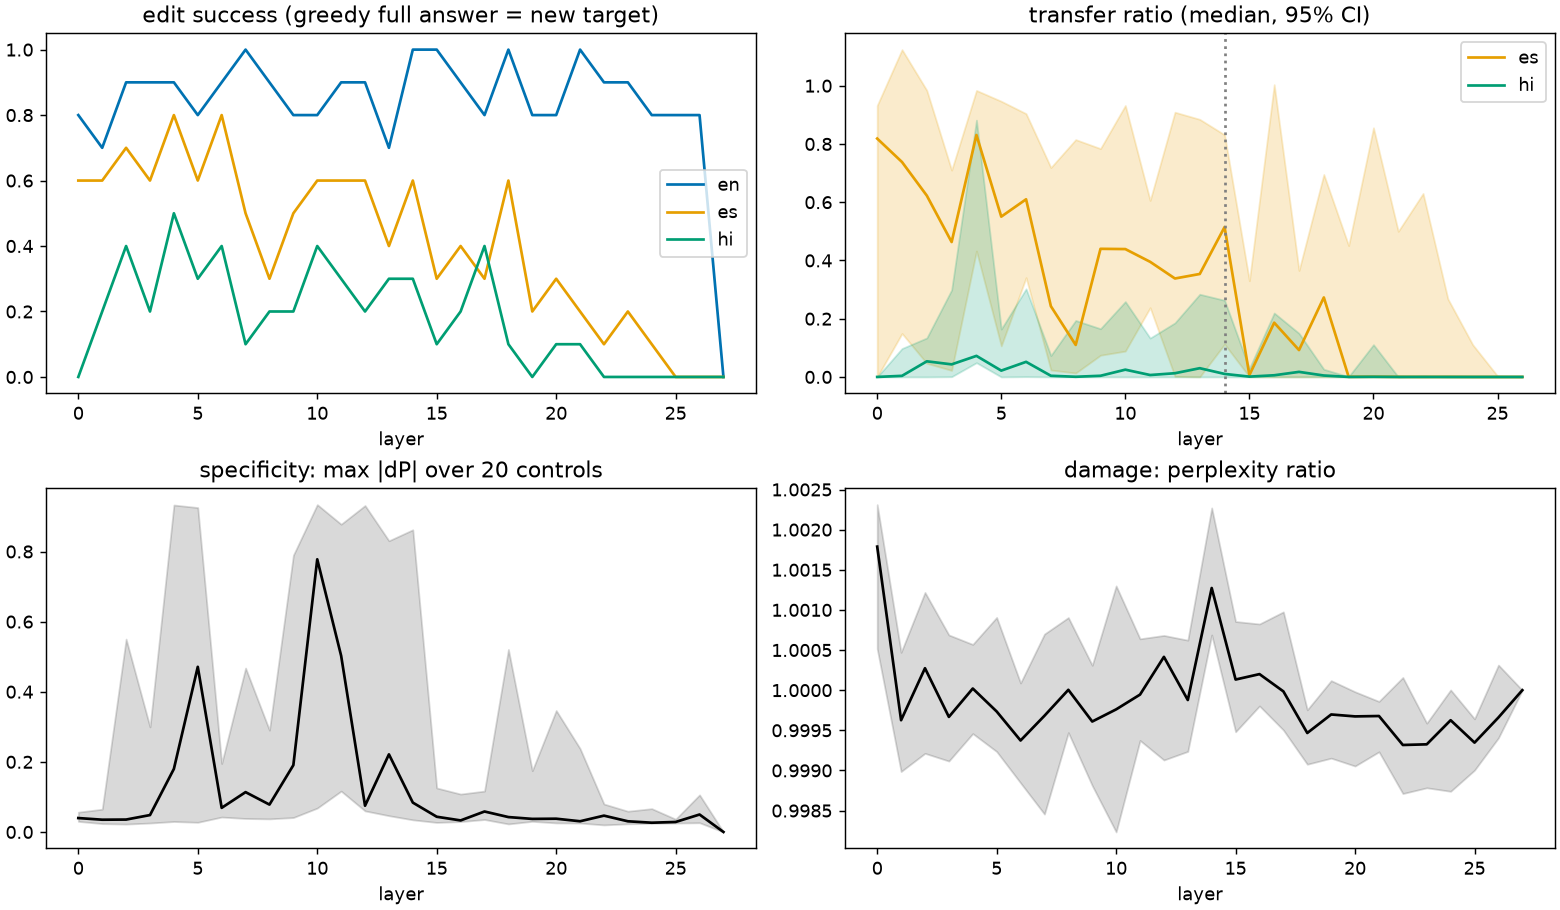
\includegraphics[width=1.0\linewidth]{figures/fig5_sweep_llama.png}\caption{Llama-3.2-3B edit sweep (10 facts, every layer): English success, transfer ratio, specificity and perplexity ratio by layer.}\label{fig:sw1}\end{figure}
\begin{figure}[t]\centering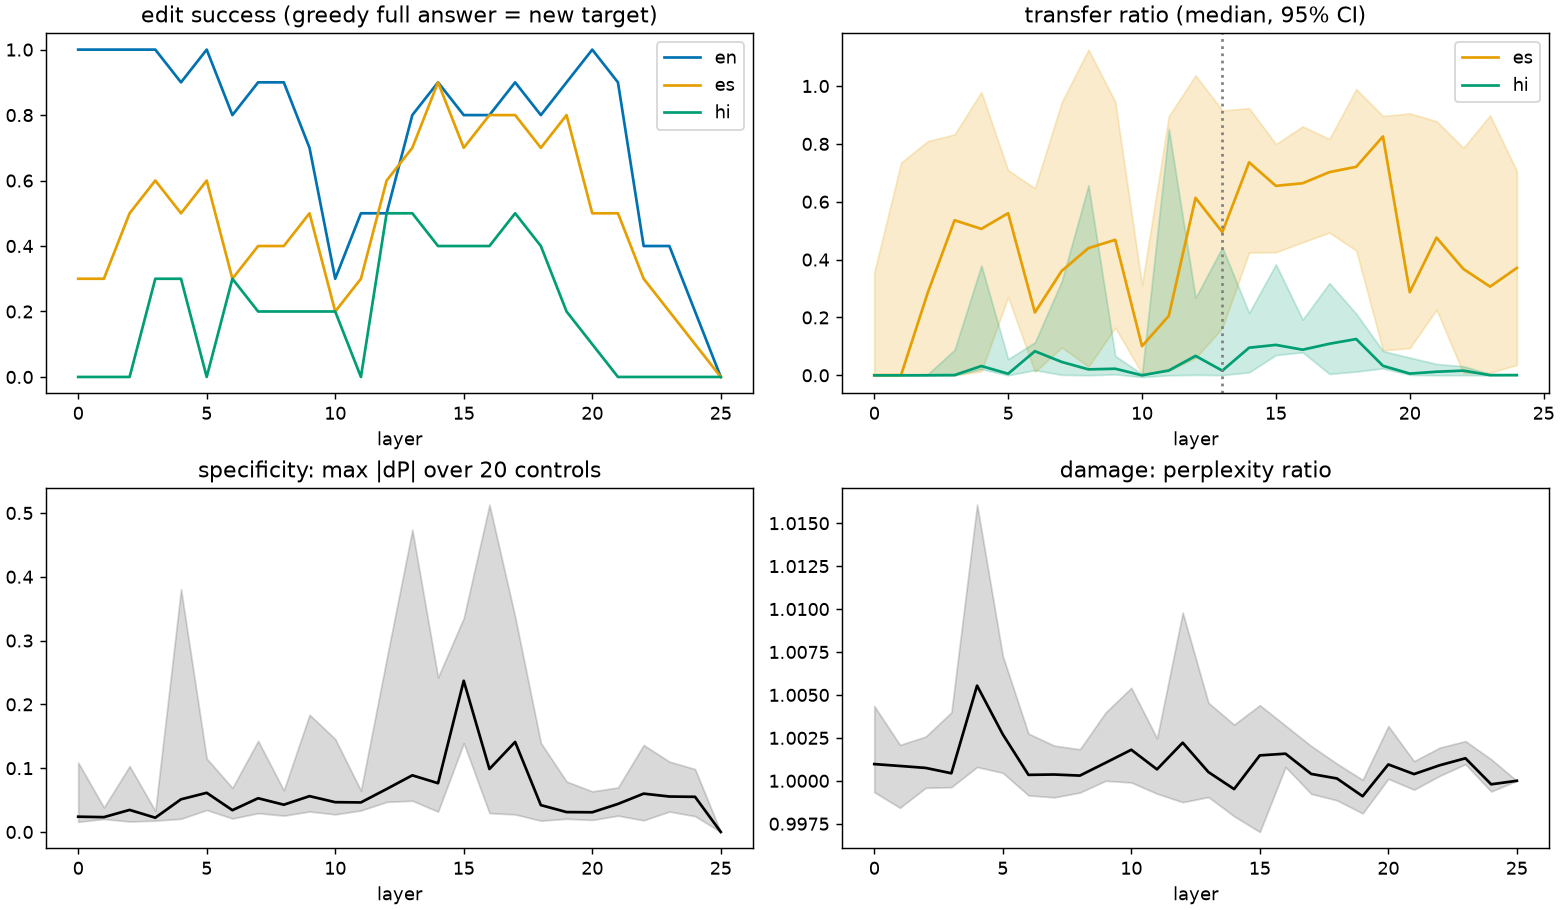
\includegraphics[width=1.0\linewidth]{figures/fig6_sweep_gemma2.png}\caption{Gemma-2-2B edit sweep, same layout as Figure~\ref{fig:sw1}.}\label{fig:sw2}\end{figure}
\begin{table}[t]\centering\small\begin{tabular}{llrcccc}\toprule
model & layer & $n$ & EN success & ES transfer & HI transfer & specificity \\\midrule
Llama-3.2-3B & traced & 10 & 0.90 & 0.664 & 0.000107 & 0.0303 \\
Llama-3.2-3B & mid & 10 & 1.00 & 0.515 & 0.0104 & 0.0838 \\
Llama-3.2-3B & random & 9 & 0.78 & 0.419 & 0.00658 & 0.0587 \\
\addlinespace
Gemma-2-2B & traced & 10 & 0.90 & 0.376 & 0.0954 & 0.0265 \\
Gemma-2-2B & mid & 10 & 0.80 & 0.495 & 0.0161 & 0.0888 \\
Gemma-2-2B & random & 6 & 0.67 & 0.0933 & 0.0364 & 0.129 \\
\addlinespace
Llama-3.2-3B, follow-up & traced & 20 & 0.80 & 0.696 & 0.00507 & 0.0624 \\
Llama-3.2-3B, follow-up & mid & 20 & 0.95 & 0.78 & 0.105 & 0.568 \\
Llama-3.2-3B, follow-up & random & 20 & 0.65 & 6.58e-05 & 2.5e-05 & 0.0281 \\
\bottomrule\end{tabular}\caption{Edit conditions: the fact's English traced layer, $L/2$ and a random layer (medians; transfer = $\Delta P_{L2}/\Delta P_{EN}$; specificity = maximum absolute probability change over 20 unrelated facts). The first two blocks are the 10-fact sweeps; the last block is the 20-fact Llama follow-up. Gemma's follow-up did not finish.}\label{tab:edit}\end{table}

\subsection{Robustness: phrasings (H8), non-copyable relations (F4), in-context baseline (F3), follow-up edits (F7)}
\emph{Phrasings (H8).} For the first 30 valid facts of each model we traced two further phrasings in all three languages. Within a language, the MLP-profile cosine between phrasings of the same fact exceeds the cross-language cosine of the canonical phrasings: Llama 0.754 against 0.609 (median per-fact difference 0.139, 95\% CI {[}0.101, 0.228{]}; 26 of 30 facts positive), Gemma 0.741 against 0.338 (0.341 {[}0.287, 0.463{]}; 30 of 30). H8 is supported in both models. By language the within-language median is 0.985 (EN), 0.744 (ES), 0.695 (HI) in Llama and 0.819, 0.778, 0.713 in Gemma. The profile therefore reflects the fact and language more than the wording, and cross-language overlap is lower than the change of wording alone.

\emph{Non-copyable relations (F4).} We added landmark\_country and city\_country, whose answers differ in form across languages. Llama keeps 34 extra facts (126 valid in total; 104 without event\_year and invention\_inventor, so the target of at least 50 is met). On the 104 non-copyable facts (Table\textasciitilde{}\ref{tab:ext}) the MLP-profile cosine is 0.653 (EN-ES, z = 4.87), 0.529 (EN-HI, z = 2.78) and 0.488 (ES-HI, z = 3.51) against a shuffled-fact null (pooled within this set). With the relation-stratified null on all 126 facts the z-values are 4.24, 2.67 and 1.98. Within single relations in Llama, EN-ES z is 2.75 (capital\_country, n = 38), 2.08 (capital\_of, 26), 1.96 (city\_country, 27) and 0.91 (event\_year, 22). Gemma keeps only one extra fact, so its non-copyable set has 29 facts and the target is not reached; there EN-ES is 0.507 (z = 2.53), EN-HI 0.314 (z = 1.16) and ES-HI 0.280 (z = 0.42). The English-Spanish alignment therefore does not depend on copyable answers in Llama; for Gemma the non-copyable sample is too small for a conclusion.

\emph{In-context baseline (F3).} On 10 facts per model we placed the new fact in an English statement before the question (descriptive, no hypothesis). In Gemma the English statement changed the answer in English for 8/10 facts, Spanish 7/10 and Hindi 6/10 (median probability change 0.48, 0.56, 0.27). In Llama it changed Spanish and Hindi answers for 10/10 facts each (0.75, 0.69) but English for 0/10 (0.003); we did not investigate this English result and draw no conclusion from it. In Llama this prompt-level transfer to Spanish and Hindi exceeds that of the weight edit (41\% and 18\% of edits on average over layers, section 4.4).

\emph{Follow-up edits (F7).} For 20 further Llama facts (30 with the sweep facts) edited at the fact\textquotesingle s traced layer, L//2 and a random layer, English success is 0.80, 0.95 and 0.65. Median Spanish transfer ratio is 0.70 (traced) and 0.78 (L//2), Hindi 0.005 and 0.105. Median specificity loss is 0.062 at the traced layer and 0.568 at L//2 (95\% CI {[}0.08, 0.78{]}); median perplexity changes by less than 0.05\% at the traced layer and L//2. Spanish transfer at the random layer is near zero (median ratio 6.6e-5). The same follow-up for Gemma did not finish (partial run kept on disk); H7 is not re-tested on these runs.

\subsection{Controls added after review (A11)}
An external review argued that the English-Spanish similarity could reflect generic profile shape or subject-name overlap. We pre-registered controls (A11, before computing) and ran them on the cached traces (Llama 126 facts, Gemma 59; 10,000 permutations; no new model run).

\emph{Same-language baselines.} In Gemma the same-fact EN-ES cosine is 0.424 against 0.242 for different facts of the same relation (EN-EN 0.247, ES-ES 0.234). In Llama it is 0.570 against 0.480 for different-fact EN-ES, but 0.606 for EN-EN and 0.413 for ES-ES: English profiles of different facts are more alike than English and Spanish profiles of the same fact, so in Llama the profile shape is strongly language-specific and the fact-specific increment (0.09) is a small part of the cosine.

\emph{Centred profiles.} After subtracting each language\textquotesingle s mean profile, the EN-ES median cosine is 0.284 (null 0.113, z = 3.61) in Llama and 0.410 (null 0.082, z = 5.43) in Gemma. The alignment is not an artefact of the shared mean profile.

\emph{Lexical overlap.} After removing accents and case, 36.5\% of Llama subjects and 11.9\% of Gemma subjects are identical in English and Spanish. The per-fact EN-ES cosine correlates with the similarity of the two subject strings in Llama (Spearman 0.29, permutation p \textless{} 0.001) and weakly in Gemma (0.22, p = 0.097). Split at the median similarity, Llama\textquotesingle s EN-ES alignment is z = 4.50 (uncentred) and 3.36 (centred) in the high-similarity half (n = 62) but 2.04 and 1.44 in the low-similarity half (n = 64); the centred value is below the pre-registered threshold of 2. Gemma\textquotesingle s low-similarity half gives z = 2.80 and 3.42 (n = 30). In Llama a substantial part of the EN-ES similarity is therefore associated with subject-name overlap, and the remainder is not distinguishable from zero after centring at this sample size; in Gemma it is not.

\emph{Entity dependence.} Clustering facts that share an English subject or answer (81 clusters in Llama, 56 in Gemma) leaves the 95\% CI of the median EN-ES cosine essentially unchanged (Llama {[}0.596, 0.688{]}; Gemma {[}0.323, 0.536{]}).

\section{Discussion}
\emph{What the evidence supports.} In both models the English and Spanish causal profiles of the same fact are aligned beyond a shuffled-fact null, and the alignment survives a relation-stratified null, rewording of the question (H8), and, in Llama, restriction to answers that are not copyable across languages. This is consistent with partly shared lookup for these two languages, but the lexical control (Section 4.6) shows that in Llama the alignment is concentrated in facts whose English and Spanish subject names are similar. Hindi is weaker: its overlap with English is above the pooled null in Llama (z = 2.90 on 126 facts) but not significant after the stratified null with Bonferroni correction (z = 2.67, p = 0.012), and depends on how many tokens the Hindi subject takes.

\emph{What it does not support.} Profile similarity at one token and one component is not identity of mechanism, and we found no evidence of a single language-agnostic space. Edits made in English reach Spanish for about half of the edits and Hindi rarely; transfer depends on the layer and on the model (H7 supported in Gemma, contradicted for Spanish in Llama). The in-context baseline shows that the model can use an English fact in Spanish and Hindi when it is in the prompt (Llama), so the low Hindi transfer of weight edits is not simply a lack of cross-lingual access; the edit site and the way Hindi is tokenised are alternative explanations that we have not separated.

\emph{Cost of mid-layer edits.} In Llama, edits at L//2 have higher median transfer than edits at the traced layer (Spanish 0.78 against 0.70, Hindi 0.105 against 0.005; the intervals overlap) but a much higher median specificity loss (0.57 against 0.06 on 20 facts); any transfer gain is therefore not free.

\emph{Scope.} Two model families, hand-written facts, 10 to 30 edit facts per condition and a small Gemma non-copyable sample limit generality. The BLOOM-1b7 and Llama-3.2-1B pilots (A10), which test whether the weak Hindi result is a tokenisation effect, had not run when this draft was written.

\section{Deviations from the pre-registration}
H6 (EN-ES z \textgreater{} 2 and EN-ES \textgreater{} EN-HI) holds in both models. H8 (phrasing robustness) is supported in both models. H9 (EN-ES z \textgreater{} 2 in at least two new or extended relations) is not supported: only event\_year was testable among the pre-registered relations (z = 0.91); the later city\_country relation reaches z = 1.96, just below the threshold. The F4 target of 50 non-copyable facts is met for Llama (104) and not for Gemma (29). The F7 follow-up (30 edit facts) finished for Llama only (20 new facts); the Gemma run was interrupted and its partial output is kept unused. The expected layer 8-19 peak is not met for Llama. Amendments A1-A10 (docs/HYPOTHESIS.md; A10, the BLOOM-1b7 pilot, is pre-registered but not yet run): critical-site definition; competitor from the corrupted run (v1 only); statistics definition; edit design; v2 design; matching rule; template selection after a poor first filter; Gemma pool extension; analysis rules (stratified null as primary for new data, non-copyable set, in-context baseline). The stratified null and the Hindi span split were added after seeing results and are labelled post hoc. v1 first-token results (66 facts, Llama only) are kept in \texttt{paper/paper.md} as a pilot; in v1 the Hindi pairs were at the null, which the v2 analysis shows to be sample- and metric-dependent.

\section{Limitations}
Two models, one of them a base and one an instruct model; hand-written facts; small per-relation samples; event\_year answers are digit strings that can be copied across languages and make up half of Gemma\textquotesingle s set; Hindi is hard to trace because subjects span many tokens; invention\_inventor keeps 0 facts in both models. Layer-0 edit results were not reproducible between runs (v1).

\section{Reproducibility}
Code, configs, write-once run directories, seeds, logs and a claim manifest (\texttt{results/manifest.json}, \texttt{./reproduce.sh\ verify}) are in the repository. End-to-end rerun status: see \texttt{docs/LOG.md}.
\begin{thebibliography}{99}\small
\bibitem{r0} Meng, K., Bau, D., Andonian, A., Belinkov, Y. (2022). Locating and Editing Factual Associations in GPT. \href{https://arxiv.org/abs/2202.05262}{arXiv:2202.05262}.
\bibitem{r1} Dubey, A. et al. (2024). The Llama 3 Herd of Models. \href{https://arxiv.org/abs/2407.21783}{arXiv:2407.21783}.
\bibitem{r2} Merity, S., Xiong, C., Bradbury, J., Socher, R. (2016). Pointer Sentinel Mixture Models. \href{https://arxiv.org/abs/1609.07843}{arXiv:1609.07843}.
\bibitem{r3} Geva et al. (2023). Dissecting Recall of Factual Associations in Auto-Regressive Language Models. \href{https://arxiv.org/abs/2304.14767}{arXiv:2304.14767}.
\bibitem{r4} Meng et al. (2022). Mass-Editing Memory in a Transformer. \href{https://arxiv.org/abs/2210.07229}{arXiv:2210.07229}.
\bibitem{r5} Hase et al. (2023). Does Localization Inform Editing? Surprising Differences in Causality-Based Localization vs. Knowledge Editing in Language Models. \href{https://arxiv.org/abs/2301.04213}{arXiv:2301.04213}.
\bibitem{r6} Gupta et al. (2024). Rebuilding ROME: Resolving Model Collapse during Sequential Model Editing. \href{https://arxiv.org/abs/2403.07175}{arXiv:2403.07175}.
\bibitem{r7} Yang et al. (2024). Understanding the Collapse of LLMs in Model Editing. \href{https://arxiv.org/abs/2406.11263}{arXiv:2406.11263}.
\bibitem{r8} Wendler et al. (2024). Do Llamas Work in English? On the Latent Language of Multilingual Transformers. \href{https://arxiv.org/abs/2402.10588}{arXiv:2402.10588}.
\bibitem{r9} Fierro et al. (2024). How Do Multilingual Language Models Remember Facts? \href{https://arxiv.org/abs/2410.14387}{arXiv:2410.14387}.
\bibitem{r10} Zhang et al. (2024). Multilingual Knowledge Editing with Language-Agnostic Factual Neurons. \href{https://arxiv.org/abs/2406.16416}{arXiv:2406.16416}.
\bibitem{r11} Wang et al. (2025). Lost in Multilinguality: Dissecting Cross-lingual Factual Inconsistency in Transformer Language Models. \href{https://arxiv.org/abs/2504.04264}{arXiv:2504.04264}.
\bibitem{r12} Lu et al. (2025). Paths Not Taken: Understanding and Mending the Multilingual Factual Recall Pipeline. \href{https://arxiv.org/abs/2505.20546}{arXiv:2505.20546}.
\bibitem{r13} Schut et al. (2025). Do Multilingual LLMs Think In English? \href{https://arxiv.org/abs/2502.15603}{arXiv:2502.15603}.
\bibitem{r14} Jiang et al. (2020). X-FACTR. \href{https://arxiv.org/abs/2010.06189}{arXiv:2010.06189}.
\bibitem{r15} Kassner et al. (2021). Multilingual LAMA. \href{https://arxiv.org/abs/2102.00894}{arXiv:2102.00894}.
\bibitem{r16} Wang et al. (2023). Cross-Lingual Knowledge Editing in Large Language Models. \href{https://arxiv.org/abs/2309.08952}{arXiv:2309.08952}.
\bibitem{r17} Khandelwal et al. (2024). Cross-Lingual Multi-Hop Knowledge Editing. \href{https://arxiv.org/abs/2407.10275}{arXiv:2407.10275}.
\bibitem{r18} Nie et al. (2024). BMIKE-53: Investigating Cross-Lingual Knowledge Editing with In-Context Learning. \href{https://arxiv.org/abs/2406.17764}{arXiv:2406.17764}.
\bibitem{r19} Qi et al. (2023). Cross-Lingual Consistency of Factual Knowledge in Multilingual Language Models. \href{https://arxiv.org/abs/2310.10378}{arXiv:2310.10378}.
\bibitem{r20} Banerjee et al. (2024). Breaking Boundaries: Investigating the Effects of Model Editing on Cross-linguistic Performance. \href{https://arxiv.org/abs/2406.11139}{arXiv:2406.11139}.
\bibitem{r21} Beniwal et al. (2024). Cross-lingual Editing in Multilingual Language Models. \href{https://arxiv.org/abs/2401.10521}{arXiv:2401.10521}.
\bibitem{r22} Durrani et al. (2025). Editing Across Languages: A Survey of Multilingual Knowledge Editing. \href{https://arxiv.org/abs/2505.14393}{arXiv:2505.14393}.
\end{thebibliography}
\end{document}
